%%%%%%%%%%%%%%%%%%%%%%%%%%%%%%%%%%%%%%%%%%%%%%%%%%%%%%%%%%%%%%%%%%%%%%%%%
% Antes de correr el código:
% 1. Ingresar al Menu
% 2. Cambiar la opción "Compiler" a XeLaTeX
% 3. Cambiar la opción "TeX live version" a 2020 (opacidad de la imagen)
%%%%%%%%%%%%%%%%%%%%%%%%%%%%%%%%%%%%%%%%%%%%%%%%%%%%%%%%%%%%%%%%%%%%%%%%%
\documentclass[10pt]{article}
\usepackage[T1]{fontenc}
\usepackage[utf8]{inputenc}
\usepackage[english]{babel}
\usepackage{listings}
\lstset{language=R}
\usepackage[a4paper]{geometry}
\usepackage[dvipsnames]{xcolor}
\usepackage[framemethod=TikZ]{mdframed}
\usepackage{graphicx,tikz}
\usepackage{array}
\usepackage{float}
\usepackage{tocloft}
\setlength{\cftsecnumwidth}{2em}
\usepackage{xspace}
\usepackage{tcolorbox}
\tcbuselibrary{listings}


% code
\usepackage{listings}
\usepackage{xcolor}

\lstset{
  basicstyle=\ttfamily\small,
  backgroundcolor=\color{gray!10},
  frame=single,
  breaklines=true,
  columns=fullflexible,
  showstringspaces=false
}

\newtcblisting{cc}{
  listing only,
  nobeforeafter,
  after={\xspace},
  hbox,
  tcbox raise base,
  fontupper=\ttfamily,
  colback=lightgray,
  colframe=lightgray,
  size=fbox
  }

\geometry{top=2.54cm, bottom=2.54cm, left=2.54cm, right=2.54cm}

\usepackage{url}
\usepackage{lipsum} 
\usepackage{wrapfig}
\usepackage{subcaption}
\usepackage{multicol}

%==========================================
%======     FUENTE PARA CÓDIGOS      ======
%==========================================
\definecolor{codegreen}{rgb}{0,0.6,0}
\definecolor{codegray}{rgb}{0.1,0.1,0.1}
\definecolor{backcolour}{rgb}{0.98,0.98,0.98}

\lstdefinestyle{mystyle}{
  backgroundcolor=\color{backcolour},   
  commentstyle=\color{codegreen},
  keywordstyle=\color{blue},
  numberstyle=\tiny\color{codegray},
  stringstyle=\color{codegreen},
  basicstyle=\ttfamily\footnotesize,
  breakatwhitespace=false,         
  breaklines=true,                 
  captionpos=b,                    
  keepspaces=true,                 
  numbers=left,                    
  numbersep=5pt,                  
  showspaces=false,                
  showstringspaces=false,
  showtabs=false,                  
  tabsize=2
}

%==========================================
%==========     ESTILO TITLE     ==========
%==========================================
\newcommand{\City}[1]{\def\City{#1}}

\makeatletter         
\renewcommand\maketitle{
\begin{flushleft}
{\textcolor{black}{\huge \bfseries \@title }}\\[1ex]
\rule{\textwidth}{0.6pt}\\
\end{flushleft}
\vspace{-0.5cm}

\begin{flushleft}
\textcolor{black}{{\large  \@author} }\\[2ex]
\end{flushleft} } % Note the extra }
\makeatother

%==========================================
%==========    ESTILO CAPTION    ==========
%==========================================
\usepackage{caption}
\captionsetup[table]{name=Tabla ,textfont={it}, labelfont={bf},
                     justification=centering,
                     width =\dimexpr \textwidth-0.5cm\relax}
\captionsetup[figure]{textfont={it}, labelfont={bf},
                      justification=centering, skip=2pt,
                      belowskip=-5pt}
                      
%==========================================
%==========     ESTILO ITEM      ==========
%==========================================
\renewcommand{\labelitemi}{$\bullet$} 
\renewcommand{\labelitemii}{$\circ$} 
\renewcommand{\labelitemiii}{$\cdot$} 

%==========================================
%===    LINKS (Agregar Hyperlinks)     ====
%==========================================
\usepackage[style=apa,
            urldate=long]{biblatex} 
\addbibresource{Bib.bib}

\DeclareSourcemap{
  \maps[datatype=bibtex]{
    \map{
      \step[fieldsource=note, final]
      \step[fieldset=addendum, origfieldval, final]
      \step[fieldset=note, null]}
      }
}

\DefineBibliographyStrings{english}{urlseen = {Accessed }    
}

\usepackage[colorlinks=true,linkcolor=RoyalBlue,
            citecolor=RoyalBlue,urlcolor=RoyalBlue]{hyperref}

%==============================================================
%==============================================================
\title{ }

%%%%%%%%%%%%%%%%%%%%%%%%%%%%%%%%%%%%%%%%%%%%%%%%%%%%%%%%%%%%%%%
%%%%%%%%%%%%                 INICIO                %%%%%%%%%%%% 
%%%%%%%%%%%%%%%%%%%%%%%%%%%%%%%%%%%%%%%%%%%%%%%%%%%%%%%%%%%%%%%
\begin{document}

\begingroup
\let\clearpage\relax % prevent extra page breaks
\thispagestyle{empty}
\begin{center}
{\huge \bfseries Universidad de los Andes}

\vspace{25pt}
{\LARGE \bfseries Departamento de Ingeniería de Sistemas}

\vspace{15pt}

\includegraphics[width=100pt]{images/logo.png} 

\vspace{35pt}
{\LARGE \bfseries Laboratorio \#3: Análisis De Capa de Transporte y Sockets}
\vspace{55pt}

{\Large \bfseries ISIS3204 - Infraestructura de Comunicaciones}


\vspace{100pt}
{\Large \bfseries Grupo 3: }

\end{center}

\begin{flushleft}
  \setlength{\parskip}{0pt}
  \setlength{\itemsep}{0pt}
  \hspace*{4cm}\large\bfseries Juan Esteban Quiroga - 202013216

  \hspace*{4cm}\large\bfseries Juan Manuel Rodriguez - 202013372

  \hspace*{4cm}\large\bfseries Andres Felipe Ortiz - 201727662
\end{flushleft}

\begin{center}
\vspace{60pt}

\Large\bfseries 2025-10
\end{center}

\mbox{}
\endgroup

\clearpage

\tableofcontents
\clearpage


\renewcommand{\thesection}{\arabic{section}}
\section*{Introducción}
\addcontentsline{toc}{section}{Introducción}
En este laboratorio implementamos un sistema de mensajería usando el modelo publicador–suscriptor con sockets TCP y UDP para simular la transmisión en tiempo real de eventos en partidos de la UEFA Champions League.  Los publicadores actúan como periodistas que envían actualizaciones en vivo de los partidos, el broker gestiona la distribución de los mensajes por partido, y los suscriptores reciben las notificaciones relevantes a las que estan suscritos. El sistema demuestra la comunicación asíncrona, la escalabilidad y los compromisos entre confiabilidad y rendimiento de los protocolos de transporte TCP y UDP en aplicaciones basadas en sockets.

\subsection*{Escenario de prueba}
Nostros creamos un sistema que permite generar simulaciones de partidos entre los siguientes equipos:
\begin{itemize}
    \item Real Madrid CF
    \item Juventus FC
    \item Paris Saint-Germain FC
    \item FC Barcelona
    \item Liverpool FC
    \item FC Bayern Munich
\end{itemize}

Sin embargo, para las pruebas realizadas en Wireshark, montamos 3 partidos en particular:
\texttt{RealMadrid\_vs\_Juventus}, \texttt{Liverpool\_vs\_BayernMunich}, y \texttt{Barcelona\_vs\_PSG} en los cuales hay un publicador por partido transmitiendo al broker. Por otro lado tenemos 4 suscriptores:

\begin{itemize}
    \item Suscriptor \#1: \texttt{RealMadrid\_vs\_Juventus}, \texttt{Liverpool\_vs\_BayernMunich}, y \texttt{Barcelona\_vs\_PSG}
     \item Suscriptor \#2: \texttt{RealMadrid\_vs\_Juventus}
     \item Suscriptor \#3: \texttt{Liverpool\_vs\_BayernMunich}
     \item Suscriptor \#4: \texttt{Barcelona\_vs\_PSG} y \texttt{Liverpool\_vs\_BayernMunich}    
\end{itemize}

\begin{figure}[H]
    \centering
    \includegraphics[width=0.75\textwidth]{screenshots/intro-1.png}
    \caption{Configuración de escenario de prueba}
\end{figure}



%==============================================================
%=======================   1   ================================
%==============================================================
\section{Modelo Publicador–Suscriptor}

\subsection{Configuración}
Nuestro proyecto tiene la siguiente configuración que fue diseñada para poder reutilizar codigo compartido entre los archivos TCP y UDP.

\begin{figure}[H]
    \centering
    \includegraphics[width=0.30\textwidth]{screenshots/intro-file-structure}
    \caption{Estructura de proyecto}
\end{figure}

\subsubsection{Compilación}

\begin{lstlisting}[language=C, caption={}]
gcc broker/src/broker_common.c broker/src/broker_tcp.c -o broker/out/broker_tcp -Wall -Wextra -std=c11 -O2

gcc broker/src/broker_common.c broker/src/broker_udp.c -o broker/out/broker_udp -Wall -Wextra -std=c11 -O2

gcc subscriber/src/subscriber_common.c subscriber/src/subscriber_tcp.c -o subscriber/out/subscriber_tcp -Wall -Wextra -std=c11 -O2

gcc subscriber/src/subscriber_common.c subscriber/src/subscriber_udp.c -o subscriber/out/subscriber_udp -Wall -Wextra -std=c11 -O2

gcc publisher/src/publisher_common.c publisher/src/publisher_tcp.c -o publisher/out/publisher_tcp -Wall -Wextra -std=c11 -O2

gcc publisher/src/publisher_common.c publisher/src/publisher_udp.c -o publisher/out/publisher_udp -Wall -Wextra -std=c11 -O2
\end{lstlisting}

\subsubsection{Ejecución}
Cada uno se corre en su propio tab en la terminal...
\\
\\
Broker
\begin{lstlisting}[language=C, caption={}]
./broker/out/broker_tcp 5050
\end{lstlisting}
Subscriber 1
\begin{lstlisting}[language=C, caption={}]
./subscriber/out/subscriber_tcp 127.0.0.1 5050 RealMadrid_vs_Juventus Liverpool_vs_BayernMunich Barcelona_vs_PSG
\end{lstlisting}
Subscriber 2
\begin{lstlisting}[language=C, caption={}]
./subscriber/out/subscriber_tcp 127.0.0.1 5050 RealMadrid_vs_Juventus
\end{lstlisting}
Subscriber 3
\begin{lstlisting}[language=C, caption={}]
./subscriber/out/subscriber_tcp 127.0.0.1 5050 Liverpool_vs_BayernMunich
\end{lstlisting}
Subscriber 4
\begin{lstlisting}[language=C, caption={}]
./subscriber/out/subscriber_tcp 127.0.0.1 5050  Barcelona_vs_PSG Liverpool_vs_BayernMunich 
\end{lstlisting}
Publisher 1
\begin{lstlisting}[language=C, caption={}]
./publisher/out/publisher_tcp 127.0.0.1 5050 RealMadrid_vs_Juventus --demo
\end{lstlisting}
Publisher 2
\begin{lstlisting}[language=C, caption={}]
./publisher/out/publisher_tcp 127.0.0.1 5050 Liverpool_vs_BayernMunich --demo
\end{lstlisting}
Publisher 3
\begin{lstlisting}[language=C, caption={}]
./publisher/out/publisher_udp 127.0.0.1 5050 Barcelona_vs_PSG --demo
\end{lstlisting}


\subsection{Publicador}
\subsubsection{Descripción}
El publicador es el componente encargado de generar y enviar los mensajes correspondientes a los eventos de cada partido. Existen dos versiones: una basada en TCP y otra en UDP, que utilizan el mismo módulo de simulación pero son distintos en la forma en que transmiten los datos.

\begin{itemize}
    \item En la versión TCP, el publicador establece una conexión confiable con el broker mediante un socket orientado a conexión. Una vez conectado, envía los eventos de forma secuencial usando la función \texttt{sendTo()}, garantizando que los mensajes lleguen en orden y sin pérdidas.
    \item En la versión UDP, el publicador utiliza un socket sin conexión, enviando cada evento mediante \texttt{send()} al puerto del broker especificado Es necesario usar esta función ya que UDP no establece un 3-way handshake entonces hay que identificar el suscriptor para enviar el evento). Aunque este método no asegura la entrega o el orden de los mensajes, permite una transmisión más rápida y ligera, simulando escenarios donde la inmediatez es prioritaria sobre la confiabilidad.
\end{itemize}

En ambos casos, los mensajes se formatean con el tema del partido y el tipo de evento, y se envían con un intervalo de aproximadamente un segundo entre ellos. 

Cada mensaje del publicador sigue el siguiente formato:

\begin{lstlisting}[language=C, caption={}]
<Match_name>|[EVENT_TYPE] <Event description> at <minute>' -- <TeamA> <scoreA>-<scoreB> <TeamB>
\end{lstlisting}

\subsubsection{Tipos de eventos}
\textbf{Estructura de partido:}

Cada partido dura 90 minutos y es dividido en 12 eventos. Para cada evento del partido, se elige un tiempo aleatorio entre rangos de valores de cada "bucket" de tiempo. Por ejemplo, el primer bucket incluye minutos del [1-7] entonces estos son posibles valores para lanzar el primer evento del partido. 
Cada uno de los 10 eventos del partido puede pertenecer a una de las siguientes categorías:
\begin{itemize}
    \item \textbf{[GOAL]} – algún jugador anota un gol y otro jugador marca la asistencia
    \item \textbf{[CARD]} – algún jugador recibe tarjeta amarilla o tarheta roja
    \item \textbf{[SUB]} – algún jugador que está jugando en el campo es reemplazado por algún jugador que está en la banca del mismo equipo y aún no ha jugado en ese partido. (solo sucede después de 55') 
    \item \textbf{[HT]} – indica el marcador en el mediotiempo (45')
    \item \textbf{[FT]} – indica el marcador final (90')
\end{itemize}
\subsubsection{Reglas de negocio}

\paragraph{Tarjetas}
\begin{itemize}
\item La primera vez que un jugador es señalado, se le muestra la tarjeta amarilla
\item La segunda vez que un jugador es señalado, se le muestra la tarjeta roja y es expulsado del partido dejando al equipo con 10 hombres en el campo
\item 20\% de las veces en cualquier evento, a un jugador se le puede mostrar una tarajeta roja directa
\end{itemize}

\paragraph{Anotar}
\begin{itemize}
\item El sistema elige uno de los dos equipos para anotar cuando se genera un evento de tipo [GOAL]
\item El jugador solo se elige si no ha sido expulsado (igual que el jugador que da la asistencia)
\end{itemize}

\subsection{Broker}
\subsubsection{Descripción}
El broker actúa como un intermediario entre los publicadores y los suscriptores dentro del sistema de notificaciones de eventos. El broker recibe los mensajes enviados por los publicadores (a través de TCP o UDP), identifica el partido al que pertenecen y los reenvia únicamente a los suscriptores que estén suscritos a ese partido.

Cada suscriptor envía un mensaje al broker que indica el interés en un partido. El broker guarda esa suscripción en una tabla interna de partidos y cada vez que llega un mensaje con ese mismo nombre de partido, lo reenvía a todos los suscriptores asociados.

(El broker no contiene lógica de negocio, ya que su función se limita al enrutamiento de mensajes. No interpreta el contenido de los eventos, ya que solo actúa como un intermediario que se encarga de que cada suscriptor reciba únicamente la información correspondiente a los partidos a los que está suscrito.)

\subsection{Suscriptor}
\subsubsection{Descripción}
El suscriptor representa al cliente final que recibe los eventos transmitidos por el sistema. Su función principal es conectarse al broker (mediante TCP o UDP) y registrarse en uno o varios temas específicos, enviando un mensaje con el siguiente formato:

\begin{lstlisting}[language=C, caption={}]
SUBSCRIBE|<topic_1> <topic_2> ... <topic_n> 
\end{lstlisting}

Una vez suscrito, el suscriptor permanece a la espera de mensajes provenientes del broker. Cada mensaje recibido tiene información sobre un evento en tiempo real que corresponde a los partidos a los que se ha suscrito.

En la versión TCP, el suscriptor mantiene una conexión persistente con el broker y recibe los mensajes mediante \texttt{recv()}. En la versión UDP, no existe una conexión formal, sino que los mensajes llegan directamente al puerto local asociado al socket mediante \texttt{recvfrom()}.

%==============================================================
%=======================   2   ================================
%==============================================================
\section{Pruebas y comparación}
En esta sección, verificamos el funcionamiento del modelo de comunicación. 
\subsection{TCP}
TCP es el protocolo que tiene envío de paquetes confiable, los mensajes llegan ordenados, y require una conexión persistente que se establece con un handshake. El flujo que sigue nuestra aplicación se describe a continuación:

\begin{enumerate}
    \item El broker crea un socket y escucha en un puerto esperando conexiones de publicadores y suscriptores. 
    \item Los suscriptores se conectan al broker por medio de conexión TCP usando el 3-way handsahke (SYN, SYN-ACK, ACK).
    \item El suscriptor manda un mensaje al broker que contiene las suscripciones que quiere.
    \item Los publicadores establecen una conexión TCP con el broker.
    \item Los publicadores envían eventos de partidos al broker.
    \item El broker identifica los suscriptores que están suscritos a los partidos asociados a los eventos que llegan de los publicadores.
    \item El broker envía los mensajes de los eventos por medio de la conexión TCP a los suscriptores.
    \item El suscriptor recibe y muestra el mensaje de cada evento.
    \item Se cierran las conexiones de los publicadores automaticamente después de enviar el último evento  (los suscriptores siguen escuchando hasta desconectarse manualmente).
\end{enumerate}

\subsubsection{Conexión suscriptores a broker}
Primero, vamos a demostrar que los suscriptores establecen un 3-way handshake con el broker. En los screenshots vemos que el suscriptor \#1 y el suscriptor \#3 hace bind con un puerto aleatorio, establace el handshake, y envía mensajes al broker indicando los partidos a los que se quiere suscribir. (para evitar redundancia solo se analizan los suscriptores 1 y 3)
\\
\\
\\
En las captura de Wireshark, los segmentos TCP con las banderas PSH y ACK indican que el emisor está enviando datos que deben entregarse inmediatamente a la aplicación receptora, sin esperar más bytes en el búfer. El campo Seq (secuencia) muestra el número del primer byte transmitido en ese segmento, mientras que Ack (acuse) confirma los bytes recibidos del otro extremo. Por ejemplo, un paquete con Seq=1 seguido de otro con Seq=34 significa que el primer mensaje contenía 33 bytes y que el segundo continúa justo después, reflejando la naturaleza secuencial y confiable de la transmisión TCP.
\\

\textbf{Suscriptor \#1 (Puerto 64376)}

\begin{figure}[H]
    \centering
    \includegraphics[width=1.0\textwidth]{screenshots/tcp-screenshots/tcp-1-handshake.png}
    \caption{Conexión de suscriptor 1}
\end{figure}

\begin{figure}[H]
    \centering
    \includegraphics[width=1.0\textwidth]{screenshots/tcp-screenshots/tcp-1-console.png}
    \caption{Verificación de conexión de suscriptor 1 en la terminal de suscriptor}
\end{figure}


\begin{figure}[H]
    \centering
    \includegraphics[width=.85\textwidth]{screenshots/tcp-screenshots/tcp-1-sus-1.png}
    \caption{Mensaje de suscripción al broker}
\end{figure}

\begin{figure}[H]
    \centering
    \includegraphics[width=1.0\textwidth]{screenshots/tcp-screenshots/tcp-1-broker-conn.png}
    \caption{Suscripciones de suscriptor 1 en terminal del broker}
\end{figure}    

\newpage
\vspace{1mm} % Add vertical space above the line
\noindent\rule{\linewidth}{0.4pt} % Draw a horizontal line across the text width
\vspace{1mm} % Add vertical space below the line

\textbf{Suscriptor \#3 (Puerto 64378)}

\begin{figure}[H]
    \centering
    \includegraphics[width=1.0\textwidth]{screenshots/tcp-screenshots/tcp-3-handshake.png}
    \caption{Conexión de suscriptor 3}
\end{figure}

\begin{figure}[H]
    \centering
    \includegraphics[width=1.0\textwidth]{screenshots/tcp-screenshots/tcp-3-console.png}
    \caption{Verificación de conexión de suscriptor 3 en la terminal de suscriptor}
\end{figure}


\begin{figure}[H]
    \centering
    \includegraphics[width=.85\textwidth]{screenshots/tcp-screenshots/tcp-3-sus-1.png}
    \caption{Mensaje de suscripción al broker}
\end{figure}

\begin{figure}[H]
    \centering
    \includegraphics[width=1.0\textwidth]{screenshots/tcp-screenshots/tcp-3-broker-conn.png}
    \caption{Suscripciones de suscriptor 3 en terminal del broker}
\end{figure}    

\vspace{1mm} % Add vertical space above the line
\noindent\rule{\linewidth}{0.4pt} % Draw a horizontal line across the text width
\vspace{1mm} % Add vertical space below the line


Cada vez que el broker detecta un partido nuevo, crea una fila en la tabla interna y si llega un suscriptor futuro que quiere recibir eventos de ese partido, solo lo asigna en la tabla.

Luego de establecer la conexión y registrar los partidos que quiere escuchar, el broker queda pendiente de mensajes con eventos de los publicadores. 

\subsubsection{Transmisión de eventos}

Como se menciona anteriormente, cada publicador también establece una conexión TCP por medio de 3-way handshake y luego envía los eventos al broker. (Por simplicidad, solo voy a detallar en Wireshark los mensajes enviados de un publicador pero al final muestro los eventos que cada publicador envió)

\textbf{Publicador \#1 (Puerto 64380)}

\begin{figure}[H]
    \centering
    \includegraphics[width=1.0\textwidth]{screenshots/tcp-screenshots/pub-1-handshake.png}
    \caption{Conexión de publicador 1 al broker}
\end{figure} 

Para evitar redundancia en el informe, adjunto un sampleo de 3 eventos (de los 12) para el partido Real Madrid vs Juventus. 

\begin{figure}[H]
    \centering
    \includegraphics[width=.85\textwidth]{screenshots/tcp-screenshots/pub-2-mensajes.png}
    \caption{Mensajes enviados al broker}
\end{figure} 

En la siguiente gráfica, muestro el log del broker de los mensajes que van llegando de los publicadores y se reenvían a los suscriptores..

\begin{figure}[H]
    \centering
    \includegraphics[width=.85\textwidth]{screenshots/tcp-screenshots/broker-event-feed.png}
    \caption{Broker logs}
\end{figure} 

En lo próxima captura, se ven todos los paquetes que recibe suscriptor 1 de los varios publicadores (mesnajes despachados por el broker)
\begin{figure}[H]
    \centering
    \includegraphics[width=.85\textwidth]{screenshots/tcp-screenshots/sus-1-rec.png}
    \caption{Mensajes recibidos por suscriptor 1}
\end{figure} 

En las capturas siguientes, se ven los mensajes generados por los publicadores:

\begin{figure}[H]
    \centering
    \includegraphics[width=.85\textwidth]{screenshots/tcp-screenshots/mad_juv.png}
    \caption{Real Madrid vs Juventus}
\end{figure} 

\begin{figure}[H]
    \centering
    \includegraphics[width=.85\textwidth]{screenshots/tcp-screenshots/liv_bay.png}
    \caption{Liverpool vs Bayern Munich}
\end{figure} 

\begin{figure}[H]
    \centering
    \includegraphics[width=.85\textwidth]{screenshots/tcp-screenshots/bar_psg.png}
    \caption{Barcelona vs PSG}
\end{figure} 

En las capturas siguientes, se ven los mensajes recibidos del broker que fueron enviados por los publicadores:


\begin{figure}[H]
    \centering
    \includegraphics[width=.85\textwidth]{screenshots/tcp-screenshots/sus-1-all.png}
    \caption{Suscriptor 1}
\end{figure} 



\begin{figure}[H]
    \centering
    \includegraphics[width=.85\textwidth]{screenshots/tcp-screenshots/sus-2-all}
   \caption{Suscriptor 2}
\end{figure} 



\begin{figure}[H]
    \centering
    \includegraphics[width=.85\textwidth]{screenshots/tcp-screenshots/sus-3-all}
    \caption{Suscriptor 3}
\end{figure} 



\begin{figure}[H]
    \centering
    \includegraphics[width=.85\textwidth]{screenshots/tcp-screenshots/sus-4-all}
    \caption{Suscriptor 4}
\end{figure} 

\subsection{UDP}
TCP es el protocolo que tiene envío de sin handshake, es más rápido que TCP pero no es confiable ya que algunos mensajes podrían no llegar o llegar fuera de orden. El flujo que sigue nuestra aplicación se describe a continuación:


\begin{enumerate}
    \item El broker crea un socket UDP y escucha en un puerto esperando conexiones de publicadores y suscriptores. 
    \item Los suscriptores crean un socket UDP y se vincula a un puerto aleatorio.
    \item El suscriptor manda un mensaje al broker que contiene las suscripciones que quiere.
    \item Los publicadores crean un socket UDP (no hay necesidad de un handshake).
    \item Los publicadores envían eventos de partidos al broker.
    \item El broker busca todos los suscriptores de los partidos según los eventos que llegan.
    \item El broker envía el evento a cada IP/puerto que corresponde.
    \item El suscriptor recibe y muestra el mensaje de cada evento.
\end{enumerate}

Primero mostramos como el suscriptor 1 manda mensajes al broker indicando a cuales partidos se va a suscribir:



\begin{figure}[H]
    \centering
    \includegraphics[width=1.0\textwidth]{screenshots/udp-screenshots/conexión_UDP.png}
    \caption{Suscriptor 1 enviando mensajes a broker en UDP}
\end{figure} 

En la próxima image, mostramos una captura del terminal del suscriptor indicando que ha enviado mensajes al broker:

\begin{figure}[H]
    \centering
    \includegraphics[width=1.0\textwidth]{screenshots/udp-screenshots/sub-1-conn.png}
    \caption{Suscriptor 1 enviando mensajes a broker en UDP (terminal)}
\end{figure} 

\begin{figure}[H]
    \centering
    \includegraphics[width=1.0\textwidth]{screenshots/udp-screenshots/sub-1-broker.png}
    \caption{Suscriptor 1 en los logs del broker}
\end{figure} 

\begin{figure}[H]
    \centering
    \includegraphics[width=.85\textwidth]{screenshots/udp-screenshots/sub-1-msj.png}
    \caption{Suscripciones enviadas al broker por suscripcion 1}
\end{figure} 

En el siguiente screenshot se ven los datos que los publicadores han enviado al broker y se han despachado a los suscriptres:

\begin{figure}[H]
    \centering
    \includegraphics[width=.85\textwidth]{screenshots/udp-screenshots/datos.png}
    \caption{Mensajes de eventos de partidos UDP}
\end{figure} 

Enseguida, estan las capturas completas de UDP:

\begin{figure}[H]
    \centering
    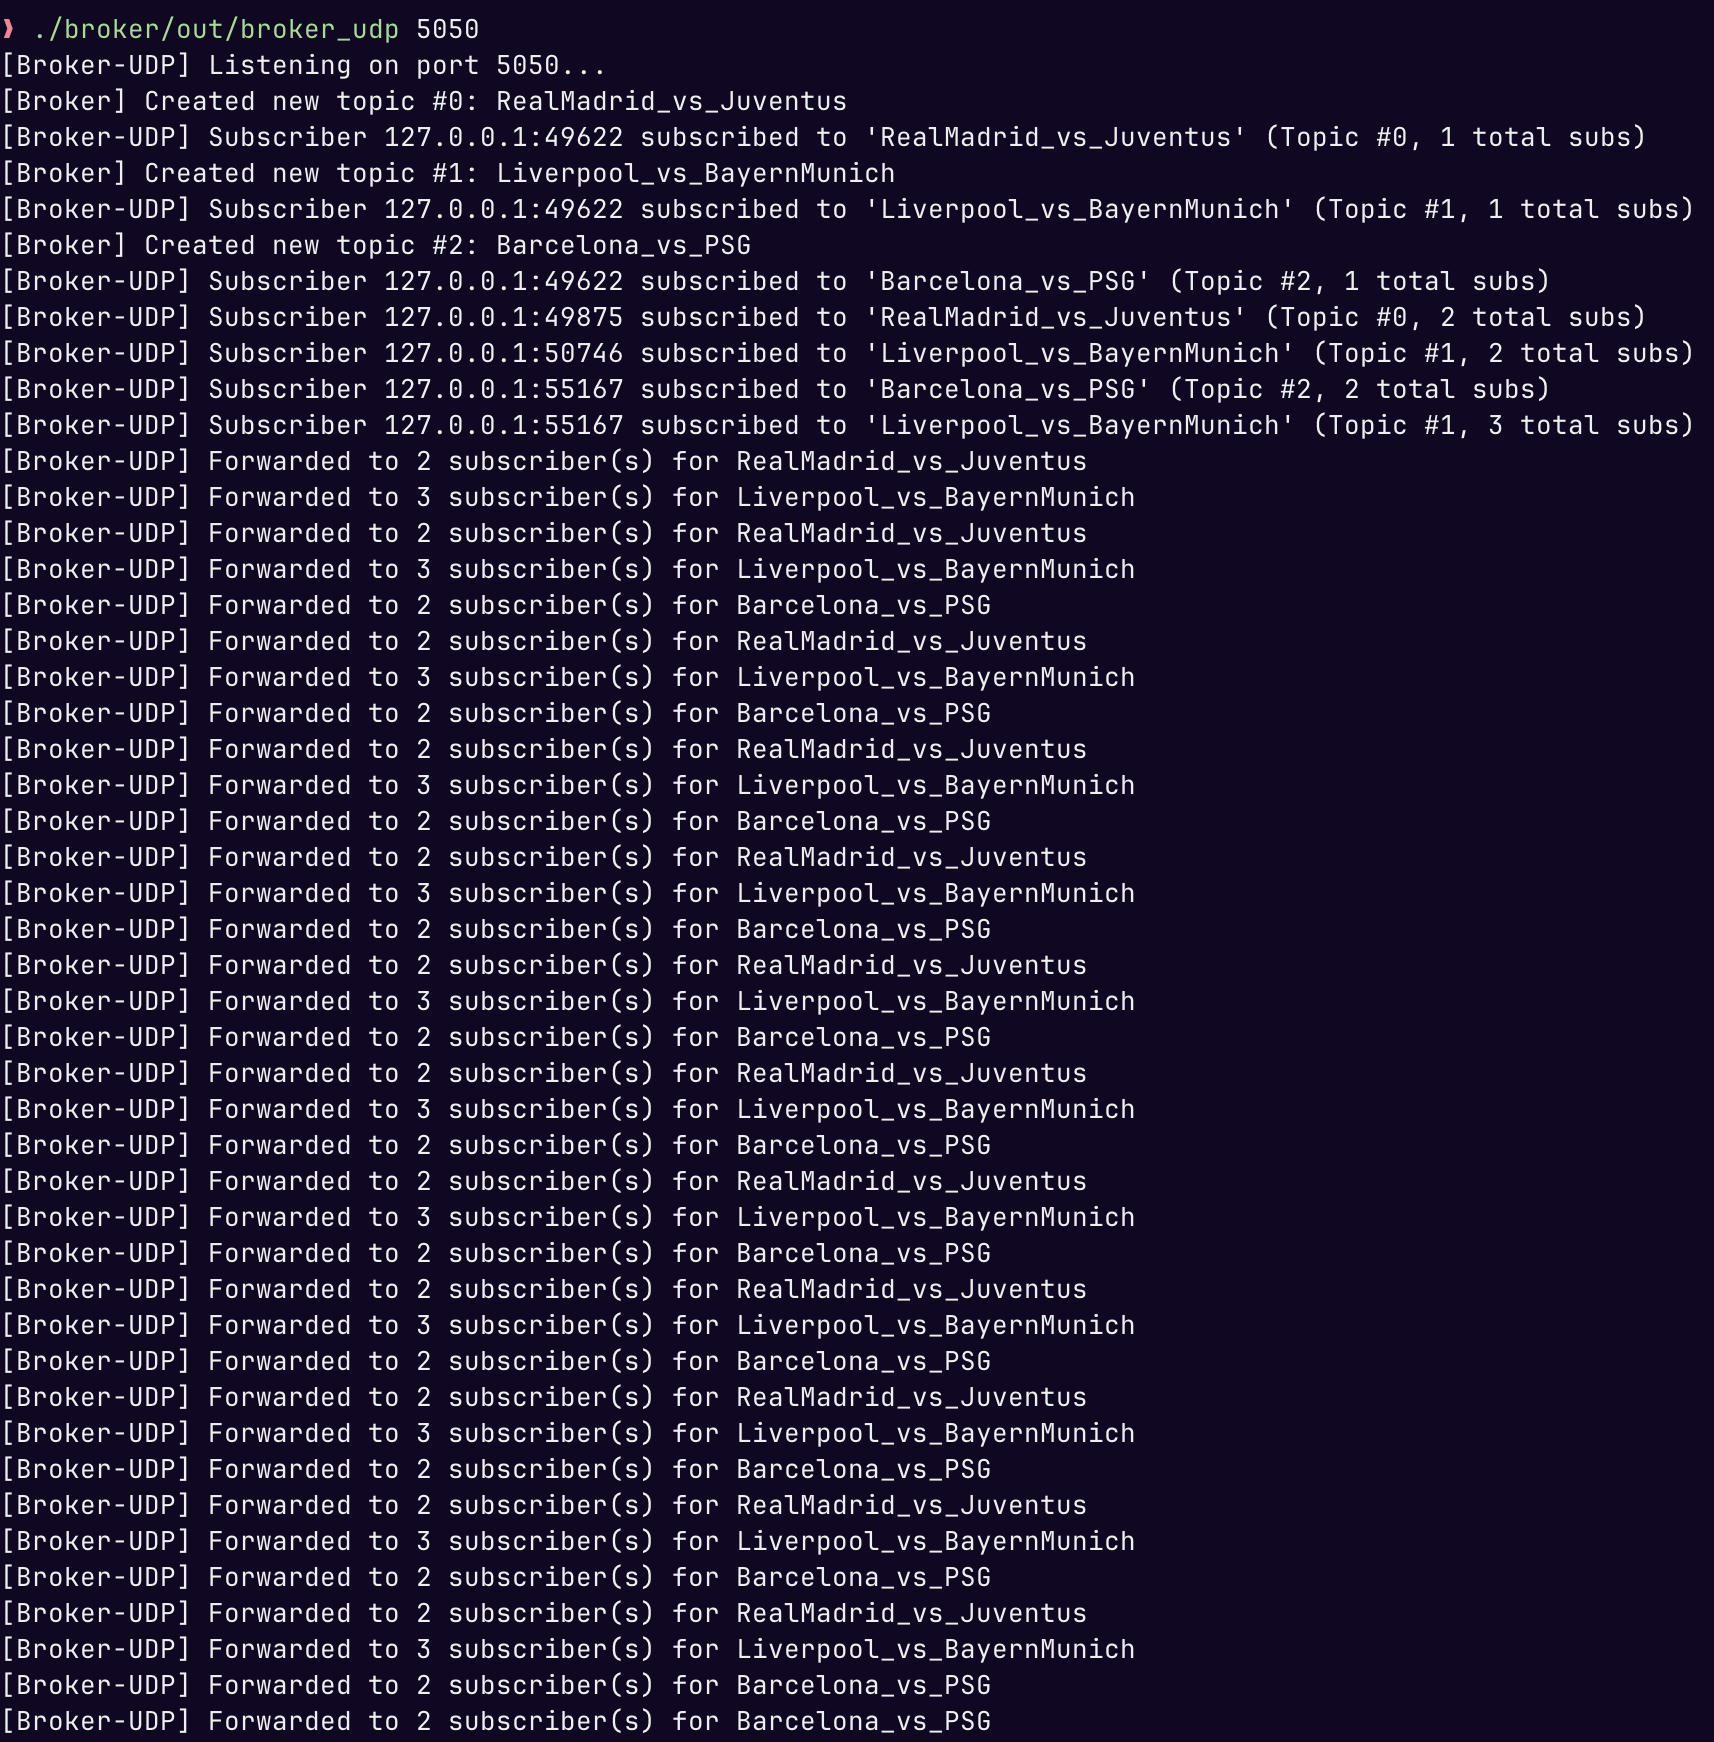
\includegraphics[width=.85\textwidth]{screenshots/udp-screenshots/broker.png}
    \caption{Log de broker completo}
\end{figure} 


\begin{figure}[H]
    \centering
    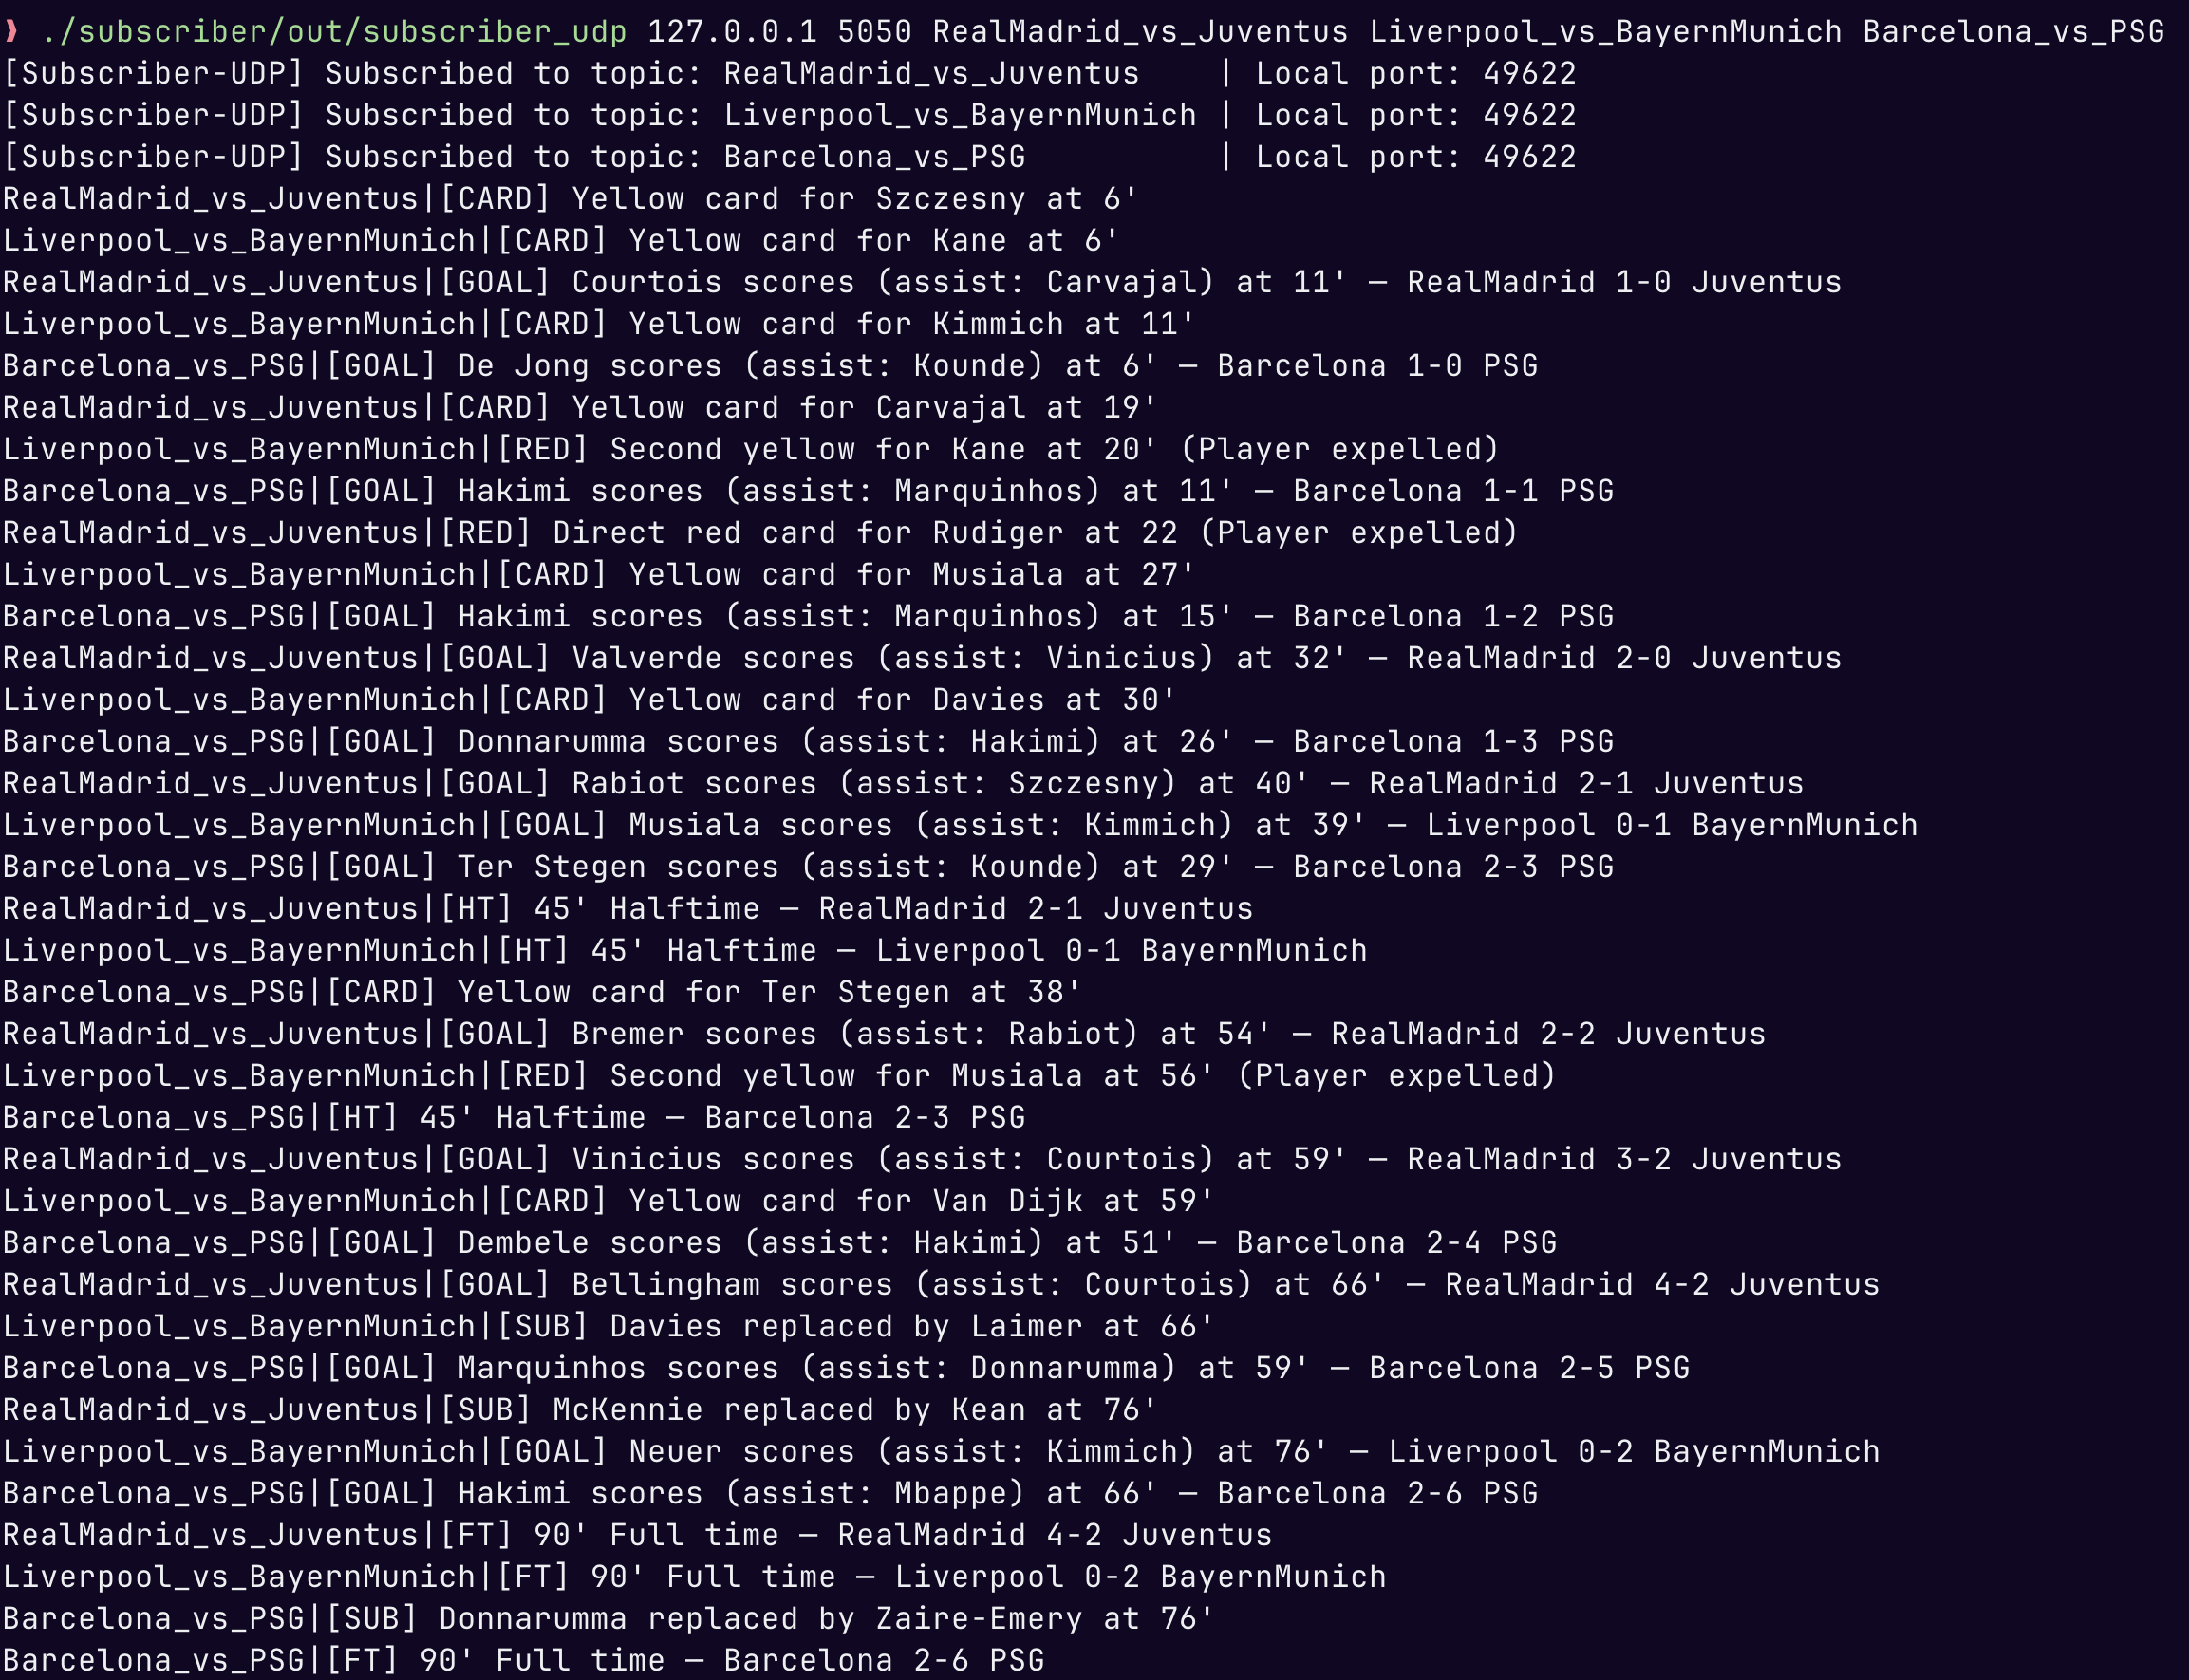
\includegraphics[width=.85\textwidth]{screenshots/udp-screenshots/sub1.png}
    \caption{Log de Suscriptor 1}
\end{figure} 

\begin{figure}[H]
    \centering
    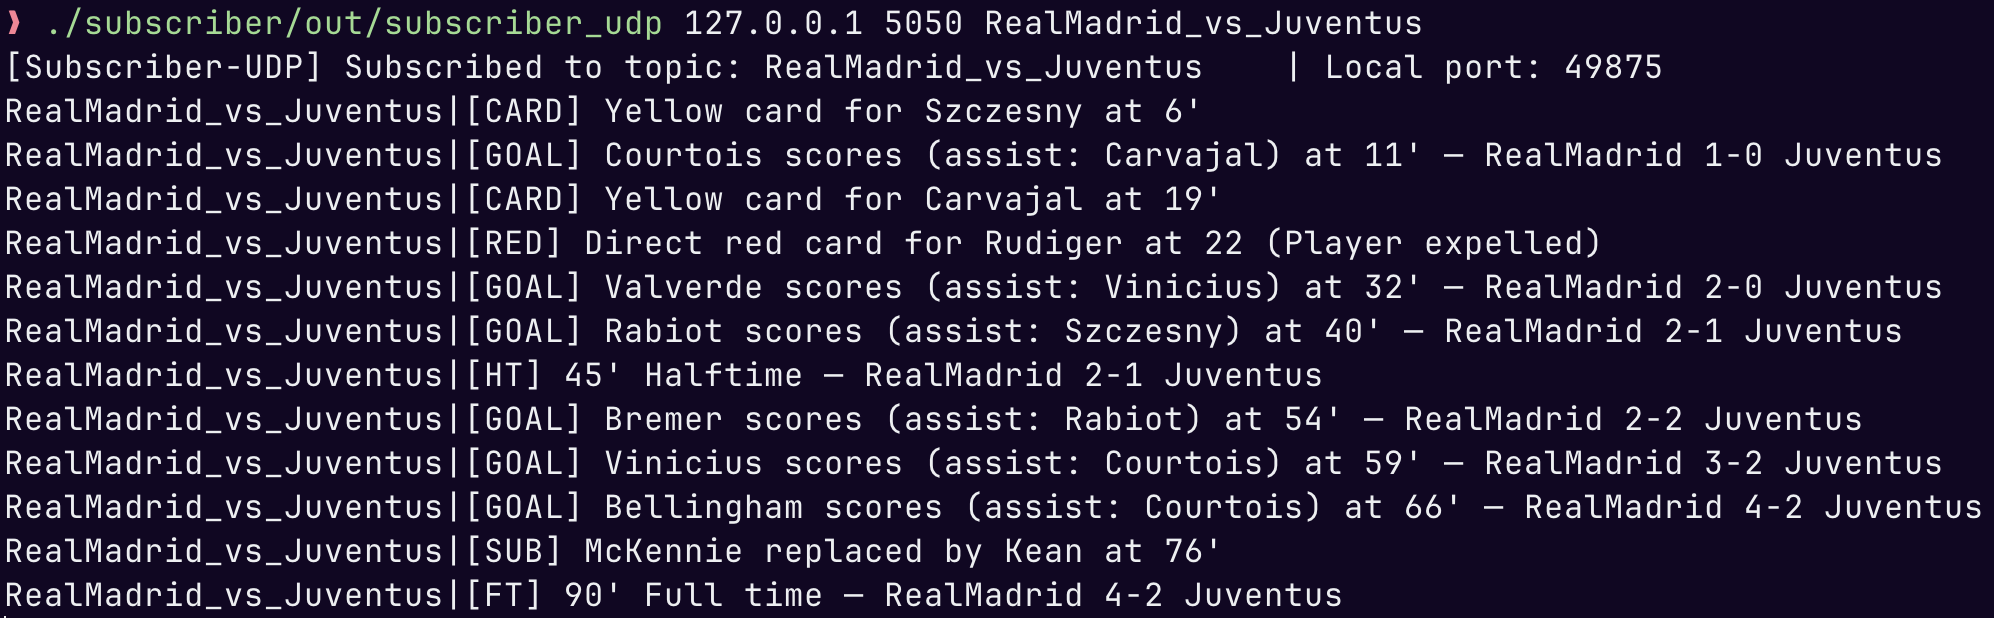
\includegraphics[width=.85\textwidth]{screenshots/udp-screenshots/sub2.png}
    \caption{Log de Suscriptor 2}
\end{figure} 

\begin{figure}[H]
    \centering
    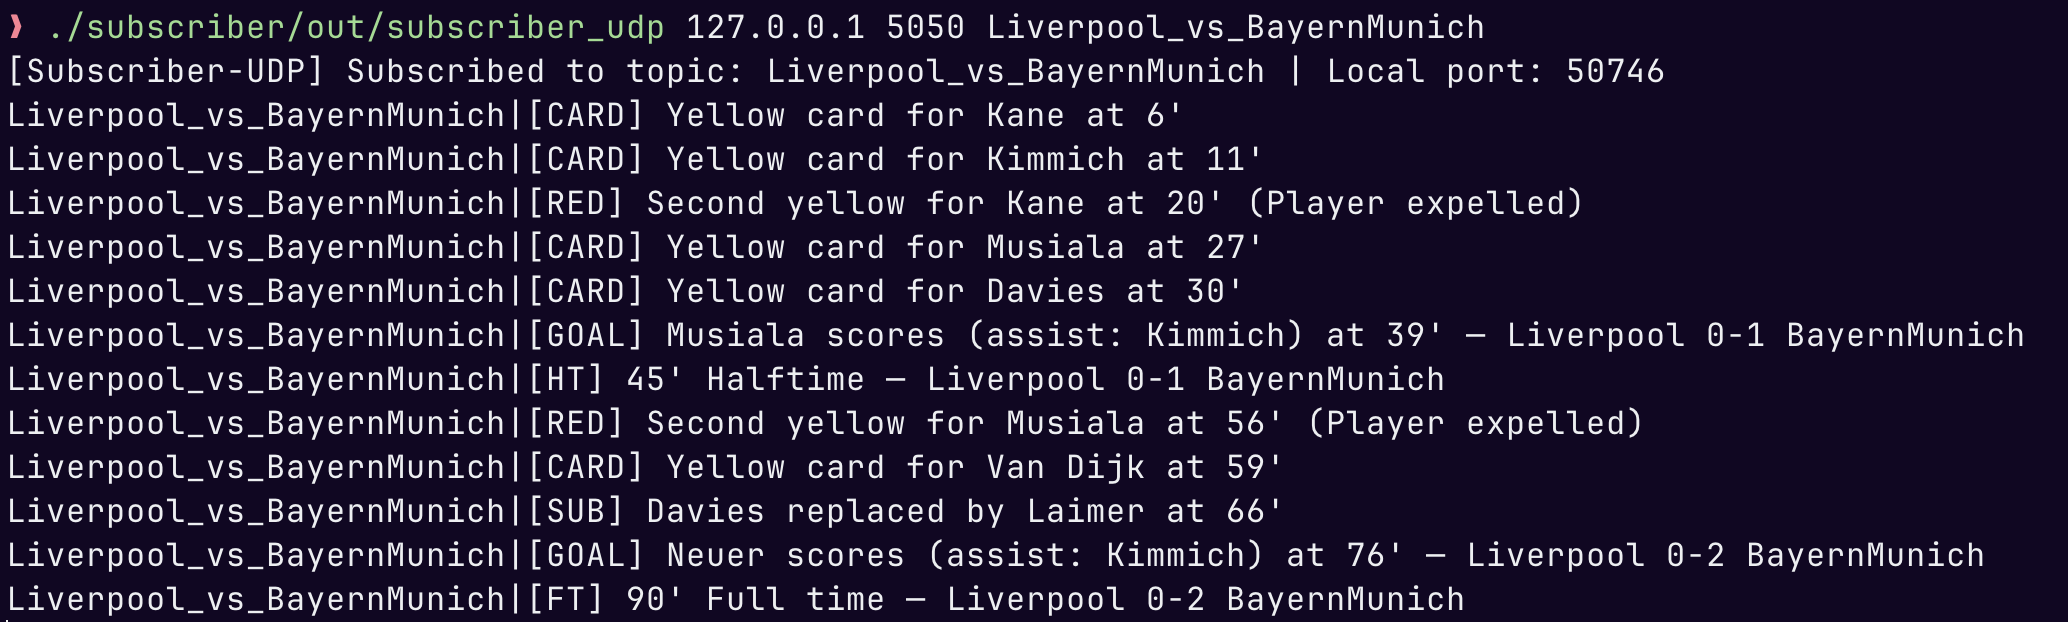
\includegraphics[width=.85\textwidth]{screenshots/udp-screenshots/sub3.png}
    \caption{Log de Suscriptor 3}
\end{figure} 

\begin{figure}[H]
    \centering
    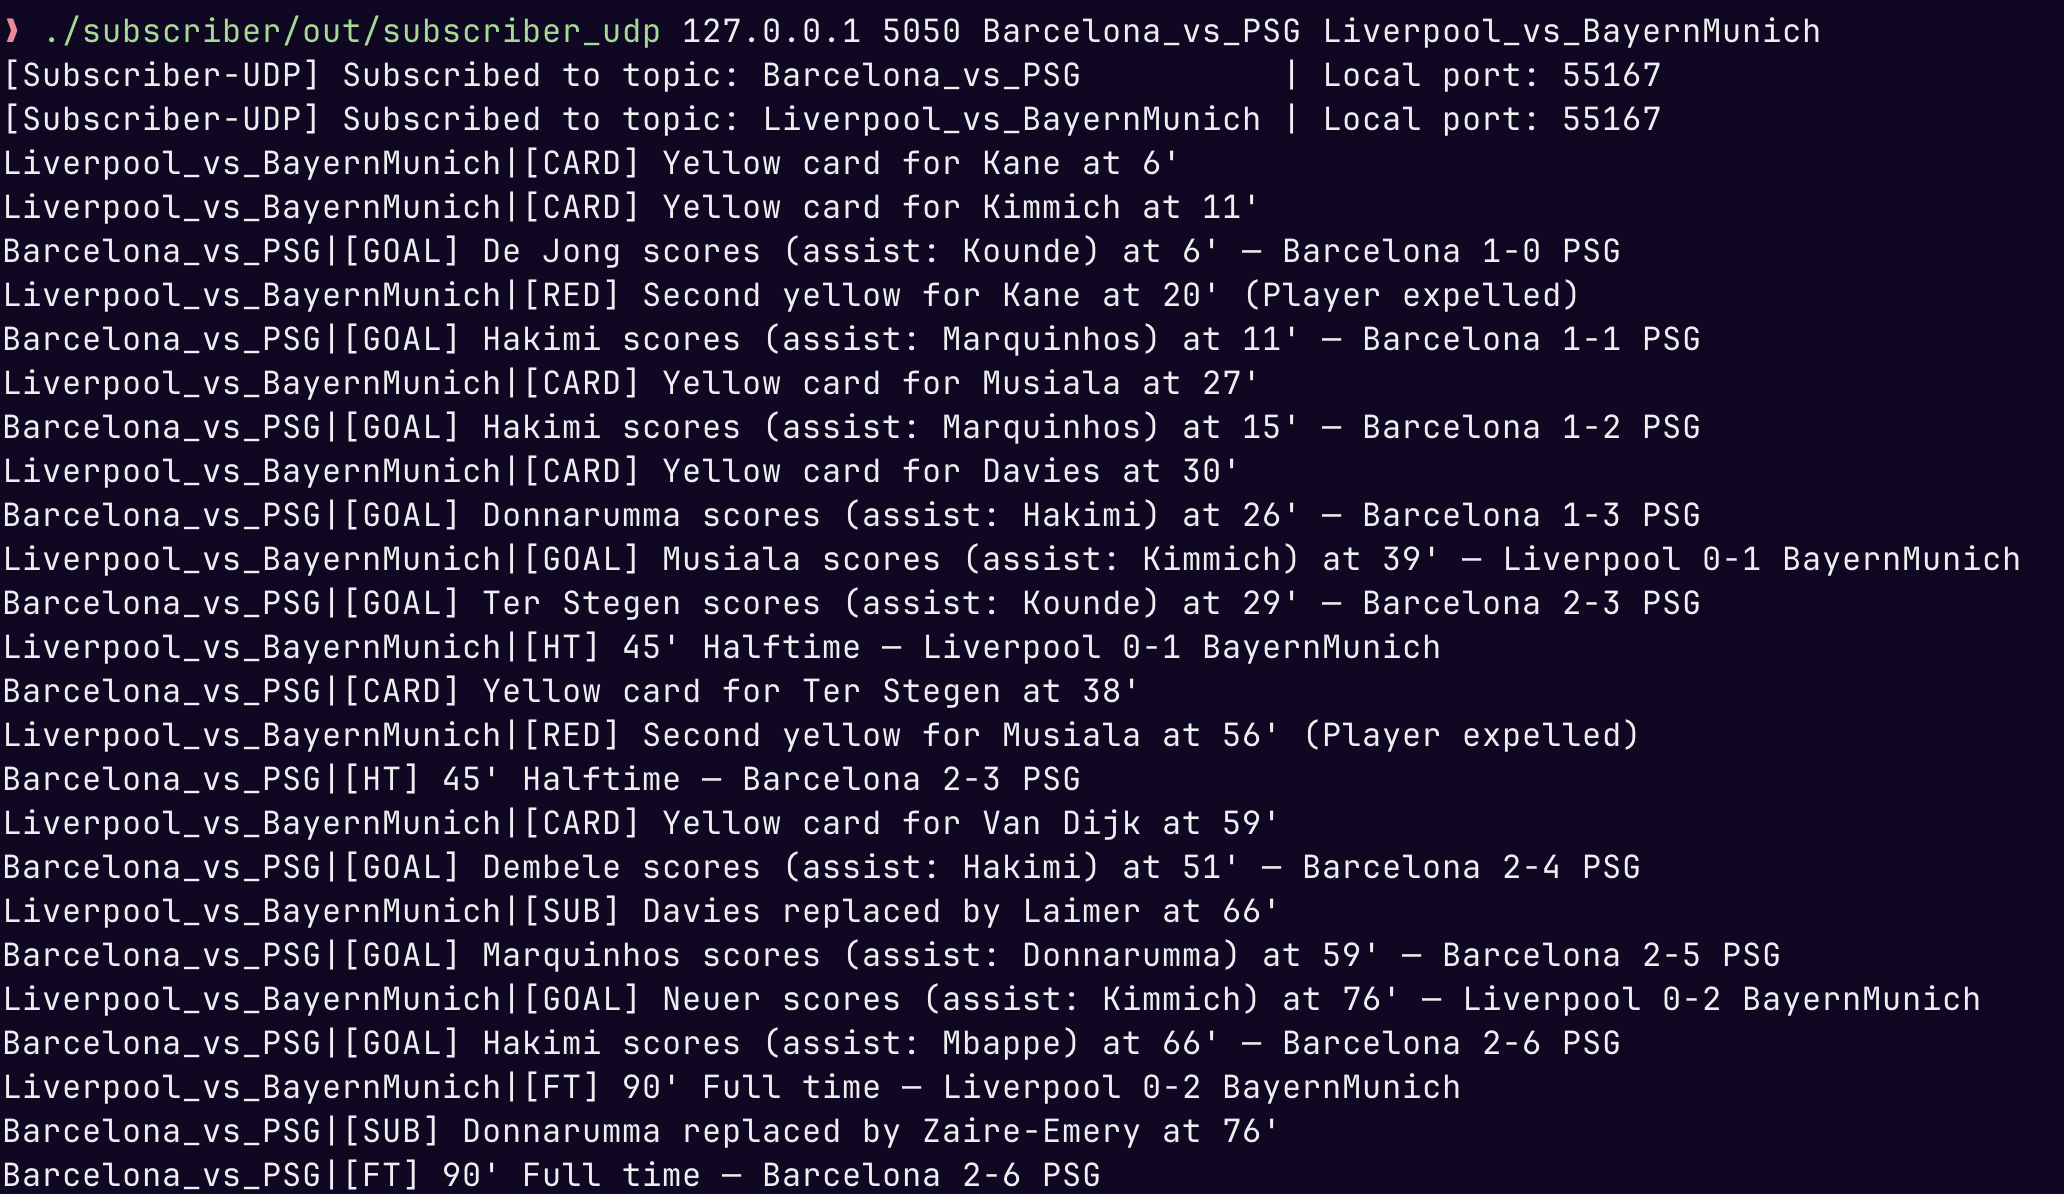
\includegraphics[width=.85\textwidth]{screenshots/udp-screenshots/sub4.png}
    \caption{Log de Suscriptor 4}
\end{figure} 

\begin{figure}[H]
    \centering
    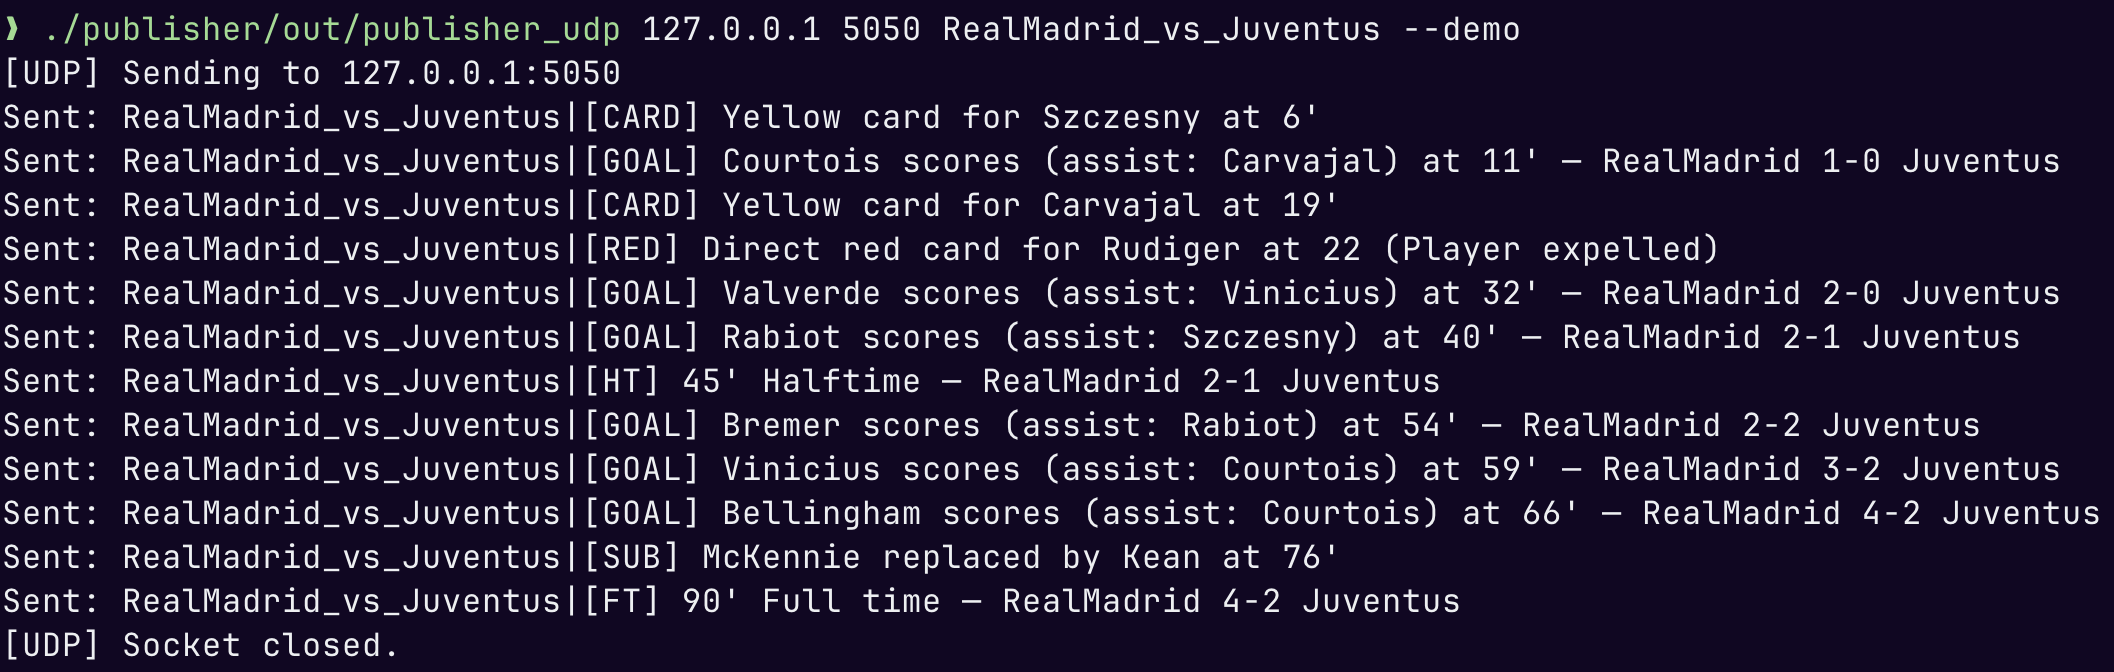
\includegraphics[width=.85\textwidth]{screenshots/udp-screenshots/pub1.png}
    \caption{Eventos de publicador 1}
\end{figure} 

\begin{figure}[H]
    \centering
    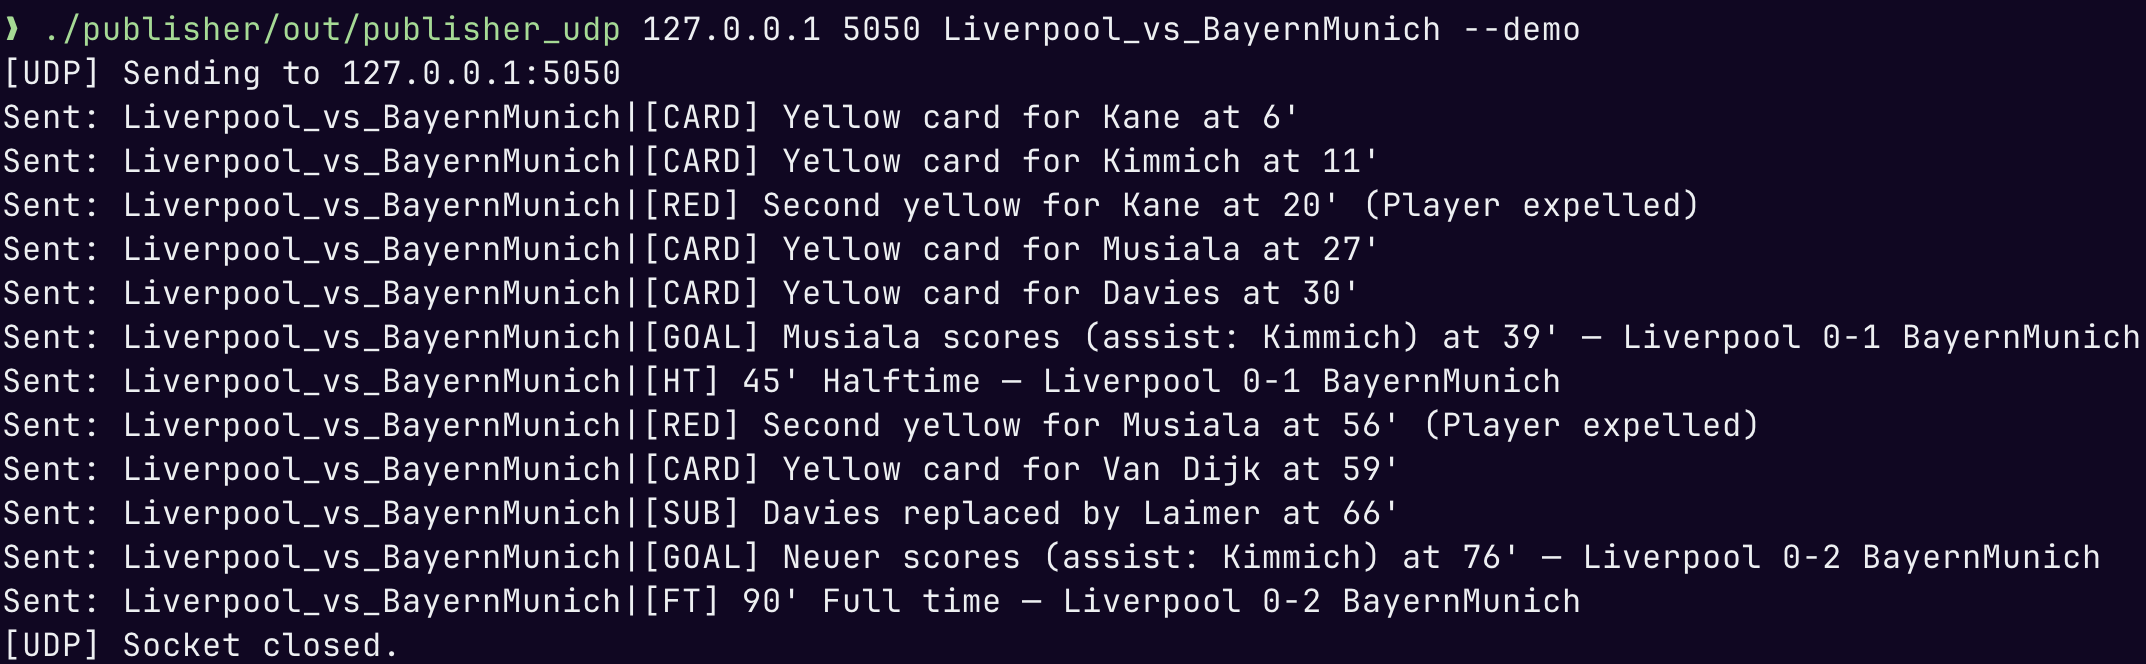
\includegraphics[width=.85\textwidth]{screenshots/udp-screenshots/pub2.png}
    \caption{Eventos de publicador 2}
\end{figure} 

\begin{figure}[H]
    \centering
    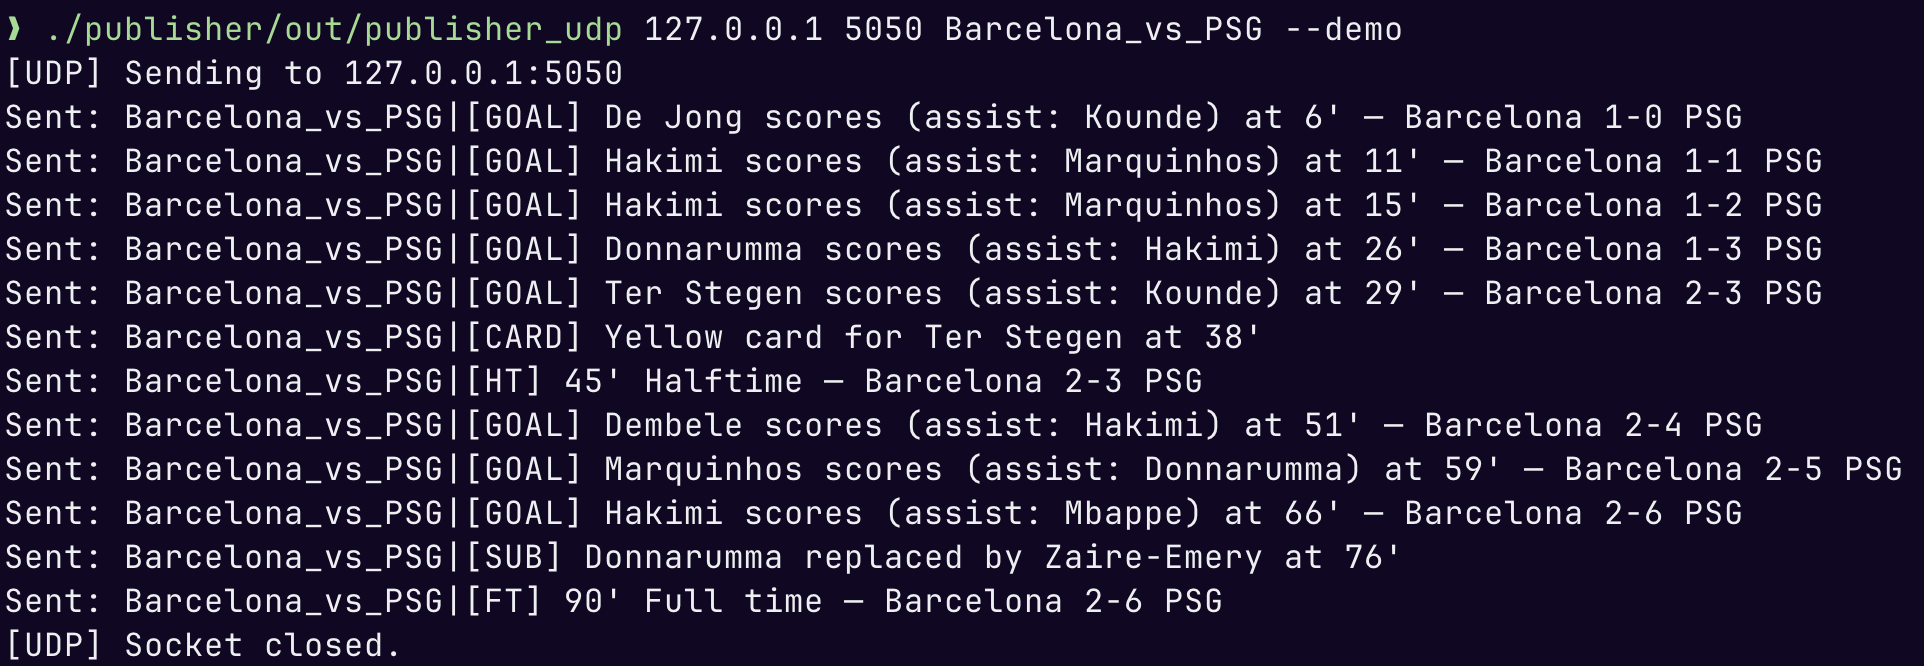
\includegraphics[width=.85\textwidth]{screenshots/udp-screenshots/pub3.png}
    \caption{Eventos de publicador 3}
\end{figure} 
























\section{Preguntas de análisis}
\section{Tabla comparativa}
\begin{table}[H]
\centering
\begin{tabular}{|l|c|c|c|c|c|c|c|}
\hline
\textbf{Protocolo} & \textbf{Total Paquetes} & \textbf{Total Bytes} & \textbf{Duración (s)} & \textbf{Paquetes/s} & \textbf{Bytes/s} & \textbf{Retransmisiones (\%)} & \textbf{Overhead (bytes)} \\ \hline
TCP & 292 & 26,773 & 24.69 & 11.83 & 1,084.27 & 47.6 & 40 \\ \hline
UDP & 149 & 16,859 & 603.64 & 0.25 & 27.93 & N/A & 28 \\ \hline
\end{tabular}
\caption{Resultados experimentales del análisis comparativo entre los protocolos TCP y UDP.}
\label{tab:tcp_udp_overhead}
\end{table}

\section{Análisis de Resultados del Laboratorio}

\subsection{¿Qué ocurriría si en lugar de dos publicadores hubiera cien partidos simultáneos?}
Si se aumentara el número de publicadores a cien, el desempeño del \textit{broker} dependería mucho del protocolo utilizado. 

Con \textbf{TCP}, cada publicador necesita su propia conexión, por lo que el \textit{broker} debe mantener información de estado, buffers y descriptores de archivo por cada una. Esto hace que el consumo de memoria y CPU crezca de forma proporcional al número de conexiones. Además, si una de ellas es lenta, puede afectar la velocidad general de entrega por los mecanismos de control de flujo.

En cambio, con \textbf{UDP} el \textit{broker} no conserva estado por conexión. Solo recibe y procesa los datagramas, lo cual permite manejar un volumen mayor de emisores con menor carga en el sistema. Sin embargo, también hay un mayor riesgo de pérdida de paquetes si la red se satura.

En resumen, TCP ofrece mayor confiabilidad, pero UDP resulta más liviano y escalable cuando el número de publicadores es muy alto.

\subsection{Si un gol se envía como mensaje y un suscriptor no lo recibe en UDP, ¿qué implicaciones tendría?}
En UDP, si un mensaje se pierde, el suscriptor simplemente no lo recibe. Esto podría generar que algunos usuarios no vean actualizaciones importantes como un gol, provocando desincronización entre los diferentes clientes.

TCP maneja mejor este tipo de situaciones, ya que garantiza que todos los mensajes lleguen al destino, aunque sea con un pequeño retraso. En una aplicación en tiempo real, la pérdida de un mensaje importante puede ser más perjudicial que un ligero aumento de la latencia, por lo que TCP sería más apropiado en este caso.

\subsection{Protocolo más adecuado para seguimiento en vivo de partidos}
La elección del protocolo depende del tipo de información que se transmite. Para eventos críticos como goles o tarjetas, lo ideal es usar \textbf{TCP}, ya que asegura que el mensaje llegue completo y en orden. En cambio, para datos que se actualizan constantemente y que pueden tolerar alguna pérdida, como estadísticas o posiciones, \textbf{UDP} es más eficiente por su baja latencia.

En las pruebas del laboratorio se observó que TCP entregó todos los mensajes de forma ordenada, mientras que UDP tuvo algunas pérdidas y reordenamientos. Por lo tanto, una solución híbrida podría ser la más adecuada en un escenario real, aunque agrega complejidad a la capa de aplicación.

\subsection{Comparación de overhead entre TCP y UDP}
El protocolo TCP utiliza más cabeceras (20 bytes de IP más 20 bytes de TCP) que UDP (20 bytes de IP más 8 bytes de UDP). Esa diferencia, aunque parezca pequeña, puede ser significativa cuando los mensajes son cortos o muy frecuentes. 

En términos de eficiencia, UDP transmite más información útil por cada paquete, pero TCP compensa su sobrecarga con la ventaja de garantizar la entrega y el orden de los datos.

\subsection{Efecto de desorden en UDP y posibles soluciones}
Cuando los mensajes llegan fuera de orden, como si primero se recibiera el marcador 2--1 y luego el 1--1, la experiencia del usuario se ve afectada y puede generar confusión. 

Para evitarlo, la aplicación puede incluir un número de secuencia o una marca de tiempo en cada mensaje, y procesarlos solo si son más recientes que el último recibido. También se pueden implementar confirmaciones (\textit{ACKs}), retransmisiones selectivas o pequeños buffers que reordenen los mensajes antes de mostrarlos. Basicamente, se termina implementando un protocolo más parecido a quic, con mayor cantidad de bits en el header del mensaje para facilitar su organizacion.

\subsection{Efecto del número de suscriptores sobre el desempeño}
Con TCP, cada suscriptor tiene su propia conexión con el \textit{broker}, por lo que al aumentar el número de suscriptores, también crece la carga en memoria y CPU y el uso del buffer por cada una de las conexiones. Además, el mismo mensaje debe enviarse de manera individual a cada cliente, lo que multiplica el tráfico.

Con UDP, el envío se realiza mediante datagramas y no se mantiene una conexión por cliente. Si la red soporta \textit{multicast}, se puede enviar una sola copia del mensaje a todos los suscriptores al mismo tiempo, lo que mejora notablemente la eficiencia. 

Basicamente, y como lo hemos mencionado anteriormente, UDP resulta mucho más rapido y eficiente, pero no es confiable como TCP.

\subsection{Comportamiento ante caída del broker}
Si el \textit{broker} se detiene, las consecuencias son diferentes según el protocolo:

Con \textbf{TCP}, las conexiones se cierran o marcan error (esto a causa de que dejara de recibir los ACK que deberia dentro de las ventanas hasta que se cumpla ese timeout designado=, y tanto publicadores como suscriptores pueden detectar rápidamente la desconexión. Sin embargo, los mensajes que no se hayan entregado se pierden si el sistema no guarda persistencia.

En cambio, con \textbf{UDP}, los publicadores seguirán enviando mensajes, pero estos se perderán sin que nadie lo note. Los clientes tampoco sabrán que el \textit{broker} dejó de funcionar.

Por lo tanto, TCP facilita la detección de fallos, aunque ninguno de los dos protocolos garantiza la recuperación automática sin mecanismos adicionales.

\subsection{Sincronización simultánea de actualizaciones críticas}
Esto es algo que es casi imposible, pues la velocidad a la que le llegan los paquetes depende de muchas fuentes de delay (delay por distancia, posibles cuellos de botella en la red de cada suscriber, etc), no solo del protocolo o de la capacidad del servidor. Teniendo esto en cuenta, se tendria que, a nivel de la capa de aplicacion ingresar logica para que ya recibido un mensaje que espere a que sea cierta hora para asegurar que a todos se les mostro de manera simultanea. 

Ahora bien, si miramos que protocolo es el que facilita la implementacion enfocandonos en la capa de transporte, el protocolo a elegir seria UDP, ya que en comparacion es mucho mas rapido que TCP, llevando que esa sensacion de sincronizacion simultanea sea mas factible de conseguir (por lo menos en aquellos que si reciben su notificacion) razon tambien por la que este protocolo es el mas utilizado en videojuegos en linea que son en tiempo real. 

\subsection{Uso de CPU y memoria en el broker}
Como lo mencionamos anteriormente, con TCP, el \textit{broker} debe mantener información de cada conexión, incluyendo buffers, estados de ventana y retransmisiones. Esto hace que el consumo de memoria crezca con el número de clientes. 

Con UDP, no se guarda información de conexión, por lo que el uso de memoria es menor. La carga de CPU proviene principalmente de la cantidad de datagramas que se deben procesar por segundo. En general, UDP tiende a ser más liviano y eficiente cuando se manejan muchos clientes.


\subsection{Diseño de un sistema real para millones de usuarios}
Para una aplicación a gran escala, lo más adecuado sería combinar ambos protocolos. 

En la comunicación entre publicadores y el \textit{broker}, se puede usar \textbf{TCP o QUIC} para asegurar que los eventos lleguen correctamente. Para distribuir la información a los usuarios finales, podría emplearse \textbf{UDP multicast} o redes de distribución de contenido (CDN) con WebSockets o HTTP/2, que mantienen buena velocidad y escalabilidad.

De esta manera, se logra un equilibrio entre fiabilidad y rendimiento: TCP asegura que la información importante no se pierda, mientras que UDP permite alcanzar una gran cantidad de usuarios con baja latencia. 

Hoy en dia es comun que las aplicaciones mas grandes, como los navegadores web o aplicaciones como facebook o X utilizan quic para las funciones para reducir la latencia en sus aplicaciones, y apoyan los procesos utilizando una fuerte logica de la capa de aplicacion.


\begin{thebibliography}{9}


  \bibitem{kurose_ross}
  Computer Networking, a top-down approach. James Kurose, Keith Ross. Addison-Wesley, 6th ed.

  \end{thebibliography}


\end{document}